\section{Background Research}
\label{section:background_research}
%%%%%%%%%%%%%%%%%%%%%%%%%%%%%%% Introduction %%%%%%%%%%%%%%%%%%%%%%%%%%%%%%%%%%%%

As of 2020, more than 50 billion devices are estimated to be using IEEE 802.11 based WiFi radios due to their low cost, robustness, and ease of use. \cite{G_Davis_2018}. The IEEE 802.11 standard, ratified in 1997, is a set of protocols for wireless communication to standardize the use of Wireless Local Area Networks (WLANs) \cite{perahia2013next}. This standardization, combined with the formation of the WiFi alliance and reduction in technological costs, led to the rapid adoption of wireless communication throughout the 2000s \cite{perahia2013next}. IEEE 802.11 made internet mobility a reality for everybody, proliferating the use of mobile technologies and paving the path for the future of communication. 

%%%%%%%%%%%%%%%%%%%%%%%%%%%%% Why mesh networking %%%%%%%%%%%%%%%%%%%%%%%%%%%%%%%%
% resilience and low power consumption emphasis

Since then, wireless communication has been evolving. Cars, drones, and traffic lights, to name a few, are all able to communicate wirelessly, each able to afford their own network requirements. Networks can be classified by their topology, which refers to the arrangement of the nodes in the network. Among others exist the hub-spoke and the mesh topology. Typically used in WiFi, the hub-spoke topology suggests the use of a central access point (AP) that acts as the gateway for all traffic within and beyond the local network \cite{ti_lethaby2017wireless}. On the other hand, a mesh network is where all devices are able to inter-communicate without the presence of a central node to organize traffic \cite{ti_lethaby2017wireless}. In mesh networks, any node(s) can act as an internet gateway \cite{ti_lethaby2017wireless}. 

\begin{figure}[H]
    \centering
    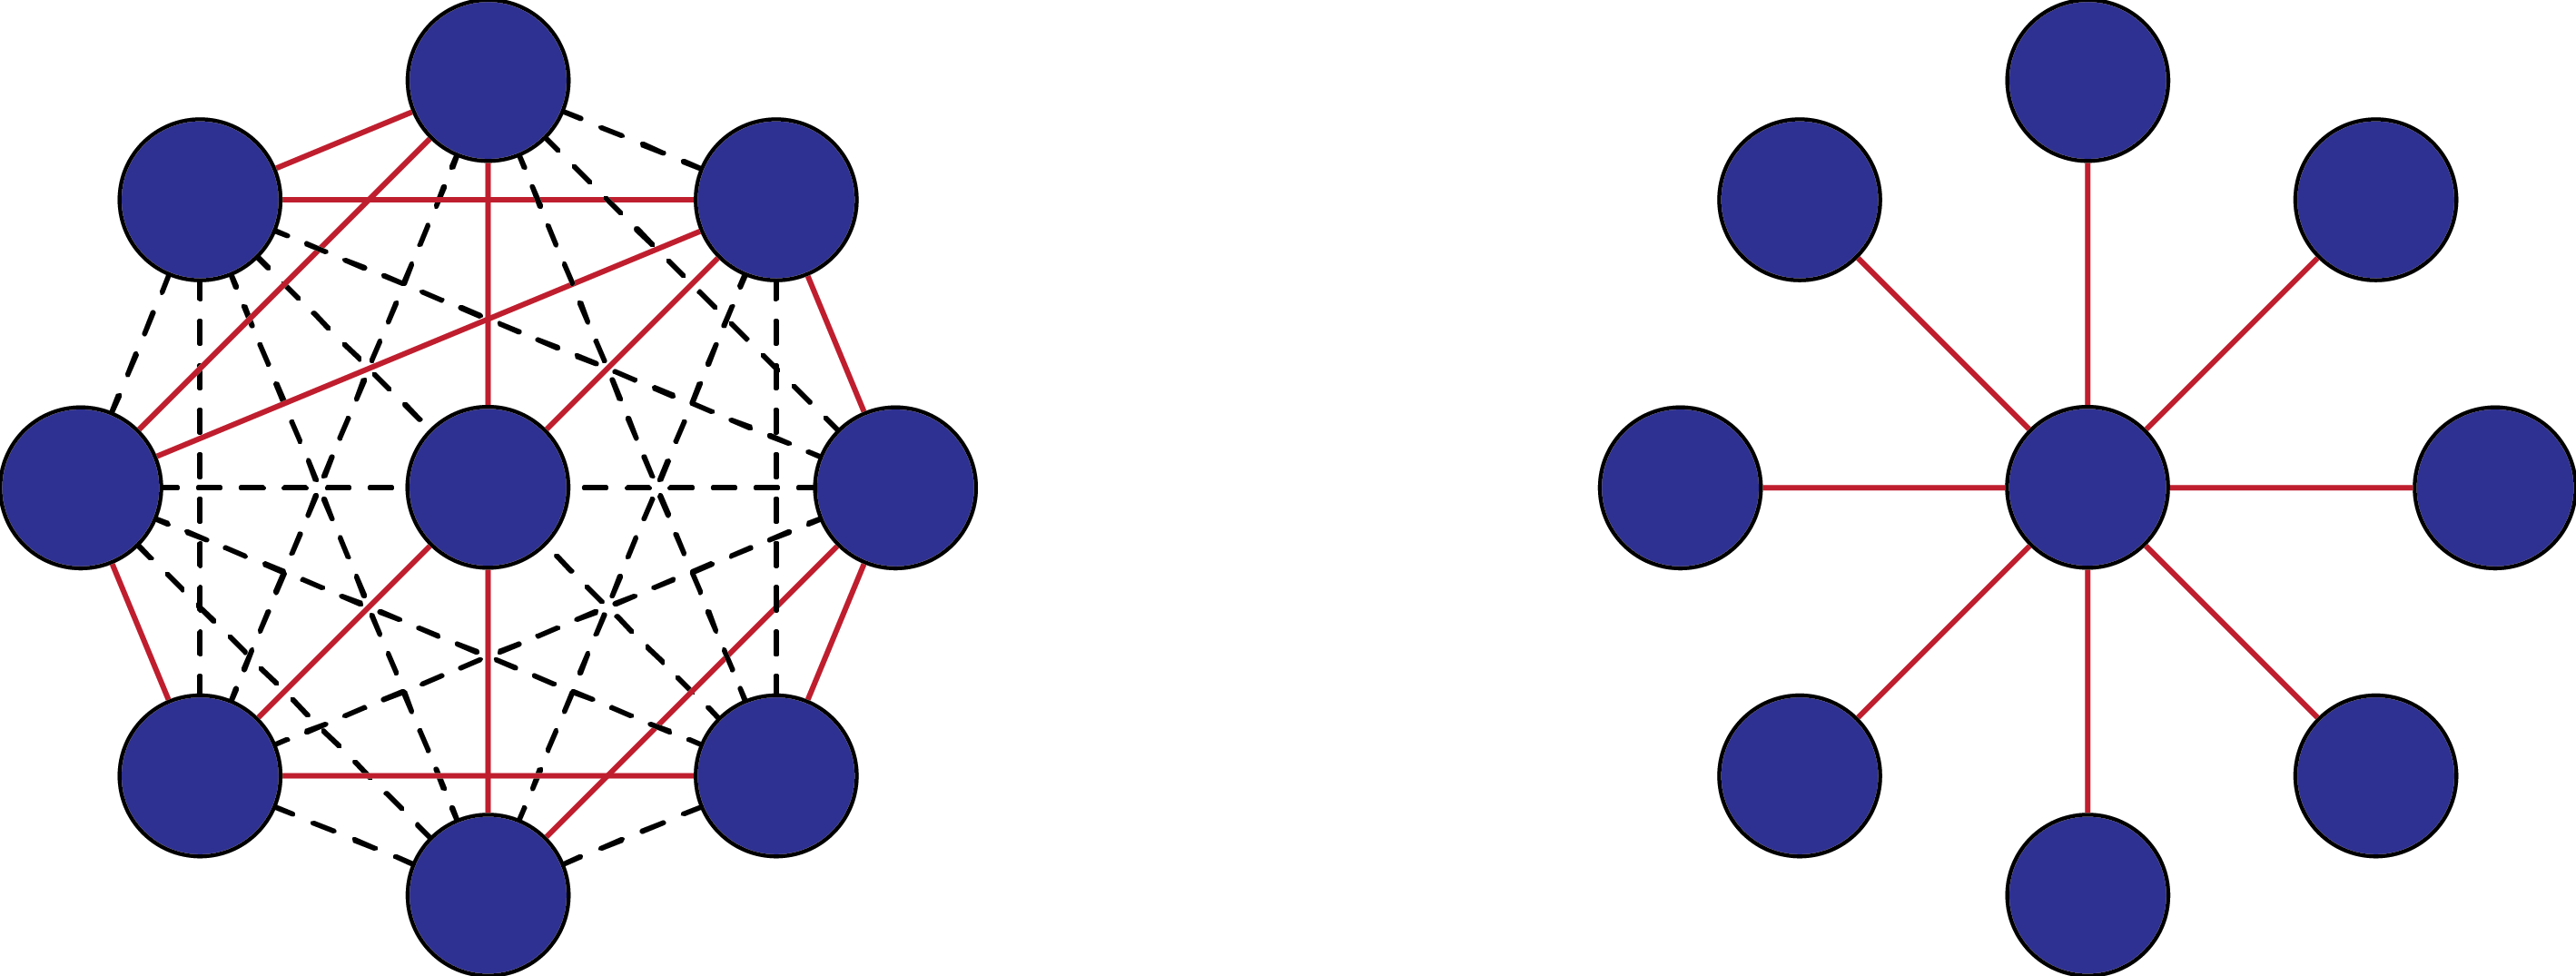
\includegraphics[width=0.6\columnwidth]{images/mesh_vs_hub_spoke.png}
    \caption{Left: A mesh network topology, Right: A hub-spoke network topology}
    \label{fig:hub_spoke_mesh_diff}
\end{figure}

While a hub-spoke topology is sufficient for typical applications, certain use cases, especially at the "internet edge" \cite{howardCoracleEvaluatingConsensus2015} requires the resilience a mesh network provides. In the case of group robotics, "centralized systems ... require a lot of computer performance from the commander" \cite{manet_drone_semenova2015network}. On the other hand, a mesh topology is "less prone to failure" \cite{manet_drone_semenova2015network} and allows for greater independence of each node. Similarly, vehicular networks require the consideration of a "highly dynamic topology" \cite{iov_wu2016internet} where nodes are moving at high speeds but also have "high-reliability requirements" \cite{iov_wu2016internet} due to safety concerns, making mesh topologies the sensible networking topology. 


%%%%%%%%%%%%%%%%%%%%%%%%%%%%% Why consensus algorithms %%%%%%%%%%%%%%%%%%%%%%%%%%%%
% resilience and dynamic topology emphasis

However, in order to meaningfully complete a task, these groups of autonomous devices must be able to coordinate and come to an agreement or a consensus. The topic of consensus is a challenging problem in distributed systems aimed at arriving at a collective agreement across all the nodes in a system, even in the presence of malfunctioning nodes \cite{Bach_Mihaljevic_Zagar_2018}. The \textit{Byzantine Generals Problem} proposed by \textit{L. Lamport} in 1982 is an analogy that aids in visualizing the need for such algorithms \cite{Lamport_1983}. According to the \textit{Byzantine Generals Problem}, a Byzantine army wants to attack a fort. Hence, each Byzantine general must decide whether to attack the target fort or retreat for protection. The caveat is that all of the generals must perform the same action simultaneously in order to minimize the number of losses. However, the generals are located at a far distance from each other and can only communicate through designated messengers, who may be lost or captured during their mission. Thus, the generals need to find a reliable way to exchange messages and reach a consensus in order to be successful. 

Consensus algorithms ensure that the critical information is reliably replicated for each node (or "generals" in the \textit{Byzantine Generals Problem}) within a system \cite{tsitsiklis1984problems}. Consensus algorithms also ensure that the nodes within the system can work as a team and succeed in their mission even if some of the nodes fail and the network topology changes \cite{raft_paper}. Therefore, consensus algorithms play a crucial role in managing a group of nodes autonomously and provide resilience against external threats \cite{Kar_Moura_2010}. Additionally, consensus algorithms provide the flexibility to add new nodes to the network, as needed, since nodes with the network can rearrange themselves autonomously \cite{Olfati_Saber_Fax_Murray_2007}. 

Similar to the \textit{Byzantine Generals Problem}, in today's world, interconnected embedded and IoT devices often need to reach a consensus in order to perform required tasks successfully and efficiently \cite{Orostica_Nunez_2019}. For example, a group of drones tasked to survey a specific area could be pre-programmed individually to complete the task. However, in such a scenario, the communication topology may be varying due to vehicle motion and communication dropouts \cite{moreau2004stability} \cite{munoz2017adaptive}. Therefore, having connectivity and consensus between these drones could drastically increase their efficiency and success rate by dynamically updating their routes based on the new information available \cite{ren2007information}. In the event of a drone loss, the remaining drones could communicate this information, and a specific drone could take over additional tasks. Furthermore, new drones could easily be added to the group as needed since the cluster can rearrange itself with the help of the consensus algorithm \cite{chen2020achieving}.


%%%%% Combining consensus algorithms and mesh networking and embedded devices %%%%% 
% Challenge of addressing problem


\begin{figure}[H]
    \centering
    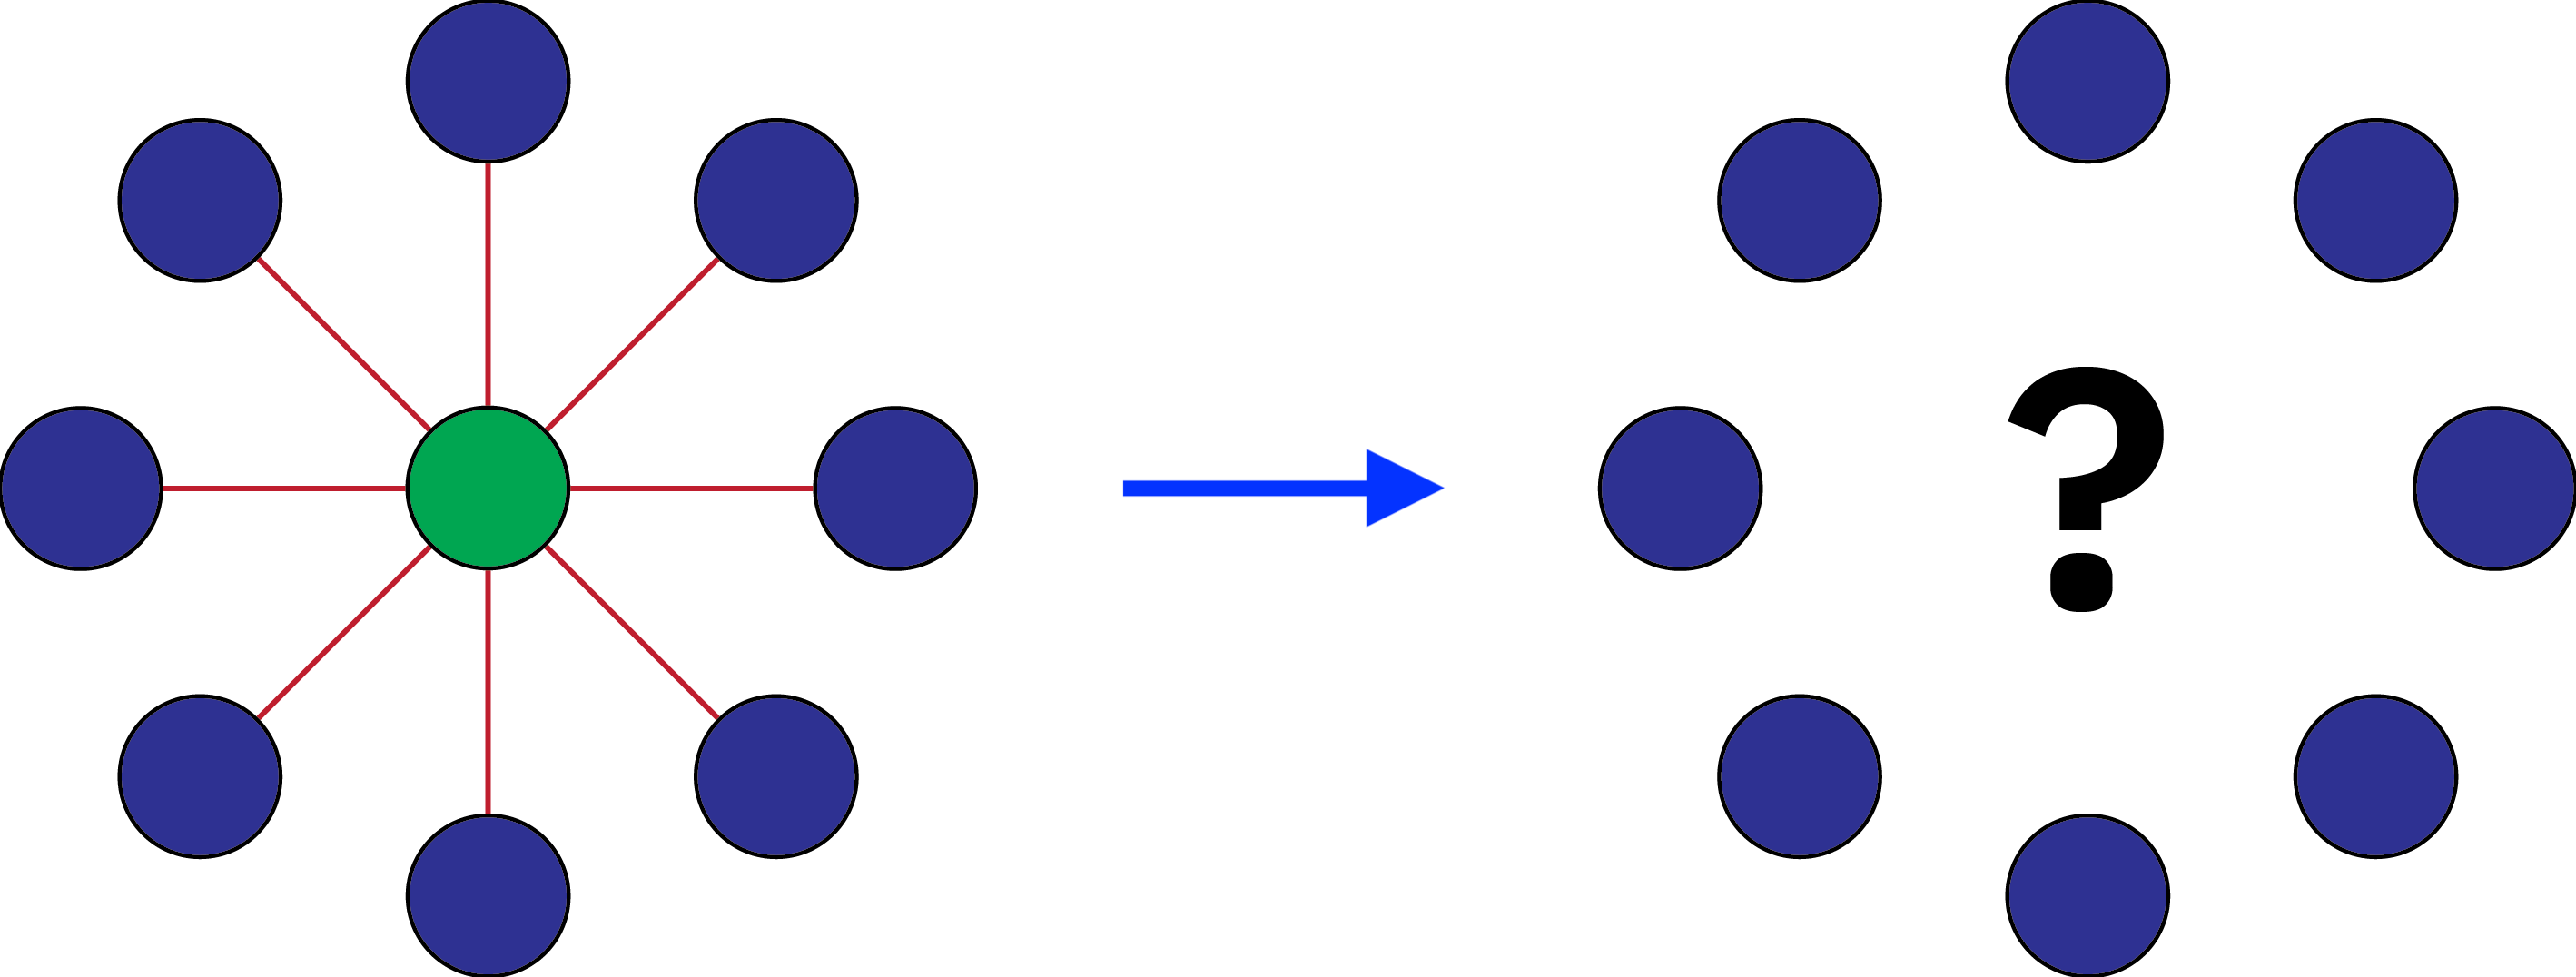
\includegraphics[width=0.6\columnwidth]{images/consensus_traditional.png}
    \caption{A consensus algorithm implemented on top of a hub-spoke network topology}
    \label{fig:consensus_traditional}
\end{figure}

A consensus algorithm could be implemented on top of traditional hub-spoke network topology, as shown in Figure \ref{fig:consensus_traditional}. The blue circles in the diagram represent the member nodes within the system, and the green circle represents the leader node. Since a hub-spoke topology is used, the green circle also represents the "hub" node in the network topology, where all of the connections meet and redistribute. A consensus algorithm implemented in this way would work without issues until there are failures stemming from the leader node. Even though consensus algorithms are capable of electing new leaders \cite{raft_paper}, the consensus algorithm would fail when the "hub" node fails in a hub-spoke network topology. This is the case because the member nodes in the system would not be able to communicate with each other to perform the election of a new leader or share information. Therefore, consensus algorithms implemented on a hub-spoke network topology are prone to a single point of failure \cite{karatas2020multi}. Given the previous drone example, if the "hub" drone fails during the mission, the rest of the cluster would not be able to communicate with each other and arrive at a consensus \cite{ren2007information}.

\begin{figure}[H]
    \centering
    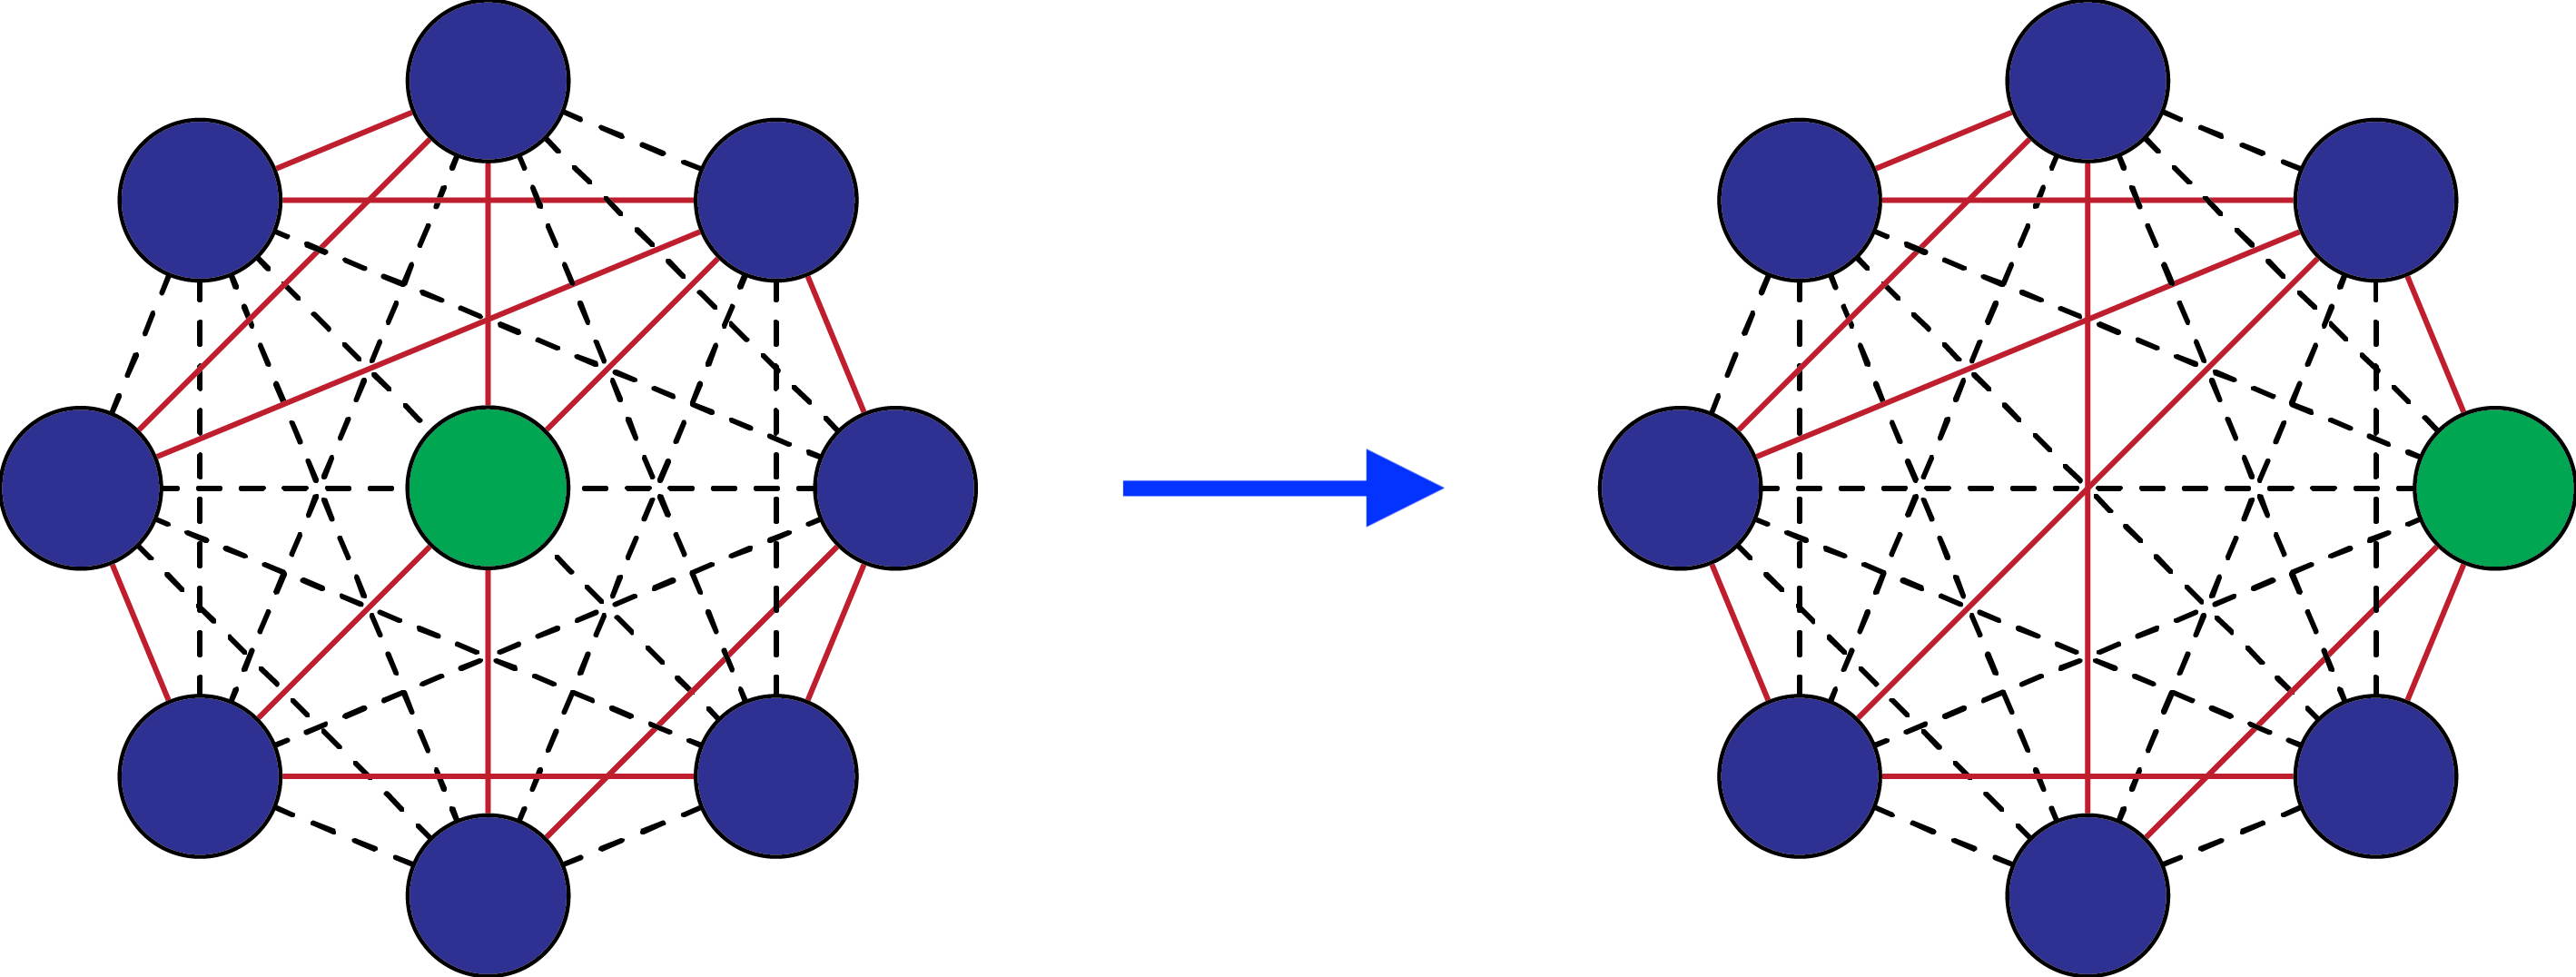
\includegraphics[width=0.6\columnwidth]{images/consensus_mesh.png}
    \caption{A consensus algorithm implemented on top of a mesh network topology}
    \label{fig:consensus_mesh}
\end{figure}

Consensus algorithms can also be implemented on top of a mesh network topology, as shown in Figure \ref{fig:consensus_mesh}. Once again, the blue circles represent the member nodes, while the green circle represents the leader node. As opposed to the implementation shown in Figure \ref{fig:consensus_traditional}, every member code can connect to each other without the need for a "hub" node. Thus, even if the leader node fails, the remaining nodes can elect a new leader node and reach a consensus. There is no single point of failure in the system shown in Figure \ref{fig:consensus_mesh}, and this situation significantly increases a system's resilience and flexibility. In light of these insights, our capstone project aims to combine mesh networking with consensus algorithms.